\documentclass[10pt,a4paper]{article}
\usepackage[utf8]{inputenc}
\usepackage{fancyhdr}
\usepackage{ngerman}
\usepackage{floatflt}
\usepackage{float}
\usepackage{graphicx}
\usepackage{tabularx}
\usepackage[ampersand]{easylist} % Aufzählung mit &
\usepackage{amsmath}
\usepackage{amsfonts}
\usepackage{amssymb}
\usepackage{array}
\usepackage{framed}
\usepackage[hidelinks]{hyperref}
\usepackage[left=3.5cm,right=2cm,top=2cm,bottom=2cm,includeheadfoot]{geometry}
\reversemarginpar
\pagestyle{fancy} %eigener Seitenstil
\setlength{\parindent}{0pt}

%Formatierung der Tabellen
\usepackage[table]{xcolor}
\renewcommand{\arraystretch}{1.3} % Zeilenabstand für Tabellen
\setlength\arrayrulewidth{0.7pt}

\usepackage{color}

%Farben für die Syntaxhervorhebung
\definecolor{pblue}{rgb}{0.13,0.13,1}
\definecolor{pgreen}{rgb}{0,0.5,0}
\definecolor{pred}{rgb}{0.9,0,0}
\definecolor{pgrey}{rgb}{0.46,0.45,0.48}

% Pakete für die Code-Formatierung von Programmcode
\usepackage{todonotes}
\usepackage{listings}
\newcommand\fnurl[2]{\href{#1}{#2}\footnote{\url{#1}}}

\renewcommand{\ttdefault}{pcr}
\lstdefinelanguage{pseudo}{
  morekeywords={if, then, else, for, in, remove, from, case, do, forever, to, return, False, True, Algorithm, Input, Output},
  literate={<=} {$\le$}{2} {!=} {$\neq$}{2} {=} {$\leftarrow$}{2} {==} {=}{2} {&&} {$\cap$}{2} {||} {$\cup$}{2},
  commentstyle=\textit,
  keywordstyle=\bfseries,
  sensitive=true,%
  morecomment=[s]{\{}{\}},%
  morestring=[b]',%
}
\lstset{language=Java,
  numbers=left,
  frame=none,
  showspaces=false,
  showtabs=false,
  breaklines=true,
  showstringspaces=false,
  breakatwhitespace=true,
  commentstyle=\color{pgreen},
  keywordstyle=\color{pblue},
  stringstyle=\color{pred},
  basicstyle=\ttfamily,
  moredelim=[il][\textcolor{pgrey}]{!!},
  moredelim=[is][\textcolor{pgrey}]{\%\%}{\%\%}
}

\lstset{literate=
  {á}{{\'a}}1 {é}{{\'e}}1 {í}{{\'i}}1 {ó}{{\'o}}1 {ú}{{\'u}}1
  {Á}{{\'A}}1 {É}{{\'E}}1 {Í}{{\'I}}1 {Ó}{{\'O}}1 {Ú}{{\'U}}1
  {à}{{\`a}}1 {è}{{\`e}}1 {ì}{{\`i}}1 {ò}{{\`o}}1 {ù}{{\`u}}1
  {À}{{\`A}}1 {È}{{\'E}}1 {Ì}{{\`I}}1 {Ò}{{\`O}}1 {Ù}{{\`U}}1
  {ä}{{\"a}}1 {ë}{{\"e}}1 {ï}{{\"i}}1 {ö}{{\"o}}1 {ü}{{\"u}}1
  {Ä}{{\"A}}1 {Ë}{{\"E}}1 {Ï}{{\"I}}1 {Ö}{{\"O}}1 {Ü}{{\"U}}1
  {â}{{\^a}}1 {ê}{{\^e}}1 {î}{{\^i}}1 {ô}{{\^o}}1 {û}{{\^u}}1
  {Â}{{\^A}}1 {Ê}{{\^E}}1 {Î}{{\^I}}1 {Ô}{{\^O}}1 {Û}{{\^U}}1
  {œ}{{\oe}}1 {Œ}{{\OE}}1 {æ}{{\ae}}1 {Æ}{{\AE}}1 {ß}{{\ss}}1
  {ç}{{\c c}}1 {Ç}{{\c C}}1 {ø}{{\o}}1 {å}{{\r a}}1 {Å}{{\r A}}1
  {€}{{\EUR}}1 {£}{{\pounds}}1
}

\makeatletter
\let\ps@plain\ps@fancy 
\makeatother

\title{InfSi3 Zusammenfassung}

\author{
	Roman Ehrbar\\
	\and
	Oliver Nietlispach
	}

\date{\today}

\begin{document}
\maketitle
\tableofcontents
\listoftodos
\newpage 

\section{Einleitung}

\subsection{Information Security Management}
Kleiner Rückblick zu den Begriffen aus InfSi1:
\begin{description}
	\item[Asset] Wert aus Sicht der Organisation, ob materiell oder immateriell, Informationen oder Dienstleistungen.
	\item[Threat] Bedrohung, möglicher Grund für einen ungewollten Vorfall, der das System oder die Organisation schädigen kann.
	\item[Vulnerabilities] Schwachstelle einer Schutzmassnahme, die durch eine oder mehrere Bedrohungen ausgenutzt werden kann.
	\item[Controls] Gegenmassnahme als Mittel zur Risikohandhabung.
	\item[Gefährdung] Zusammenspiel von Asset, Threat und Vulnerabilities.
	\item[Applied Threat] Die Gefährdung ist eine Bedrohung, die konkret über eine Schwachstelle auf ein Objekt einwirkt. (Bedrohung und Schaden)
	\item[Risiko] = Wahrscheinlichkeit eines Zwischenfalls * Schaden = Bedrohung * Verletzlichkeit * Schaden
\end{description}

\subsection{Treiber für Informationssicherheit}
Als hauptsächlicher Treiber der Informationssicherheit zählt die \textbf{Konformität zu Gesetz und Vorschriften}.

Folgendes liefert ein Teil von Gesetzen und Vorschriften in den verschiedenen Sparten:
\begin{easylist}[itemize]
	& Bearbeiter von Personendaten
	&& Diverse Strafgesetzbuch Artikel
	&& Datenschutzgesetz (DSG)
	&& US Health Insurance Portability and Accountability Act (HIPAA)
	& Finanzdienstleister
	&& Bankgesetze (Bankgeheimnis, etc.)
	&& EU Directive on Payment Services (PSD)
	&& Payment Card Industry Data Security Standard (PCI)
	& Telecom/ICT-Anbieter
	&& Fernmeldegesetz
	&& Lawful Interception
	& Allgemeines Controlling
	&& Sarbanes-Oxley Act (SOX), US-börsenkotierte Firmen
\end{easylist} 

\subsubsection{Datenschutzgesetz DSG}
\begin{quotation}
	Wer als Privatperson Personendaten bearbeitet oder ein Datenkommunikationsnetz zur Verfügung stellt, sorgt für die Vertraulichkeit, die Verfügbarkeit und die Richtigkeit der Daten, um einen angemessenen Datenschutz zu gewährleisten. - DSG Art. 8
\end{quotation}

\subsubsection{Strafgesetzbuch StGB}
\begin{quotation}
	Missbrauch einer Fernmeldeanlage - StGB Art. 179septies (Virentatbestand)
\end{quotation}

\begin{quotation}
	Unbefugtes Beschaffen von Personendaten - StGB Art. 179novies (Hackingtatbestand)
\end{quotation}

\subsubsection{Health Insurance Portability and Accountability Act HIPAA}
Umfasst mehrere Regeln zu Datenschutz und -Sicherheit von Gesundheitsdaten. Dazu wird auch eine Regel für die \textit{Unique Identifiers} definiert (National Provider Identifier, NPI).

\subsubsection{Bankengesetz BankG}
\begin{quotation}
	Der Bankkunde hat ein Recht auf Schutz seiner ökonomischen Privatsphäre, die Bank hat somit die Pflicht, über alle Tatsachen, die ihre Kunden betreffen, Verschwiegenheit zu wahren. - BankG Art. 47
\end{quotation}

\subsubsection{Payment Card Industry Data Security Standard}
Dieser umfasst mehrere Bestimmungen wie z.B. den Einsatz einer \textbf{Firewall}, \textbf{Verschlüsselte Übertragung}, \textbf{Beschränkung des physikalischen Zugriffs}, usw.

\subsubsection{Sarbanes-Oxley Act SOX}
Fordert verschärfte interne Kontrollsysteme und führt zu höheren Anforderungen an die \textit{Corporate Governance}.

\subsection{Risiken und Bedrohungen}

Für den Umgang mit Risiken können Unternehmen unterstützend ein \textbf{Information Security Management System} einsetzen.

\begin{figure}[H]
	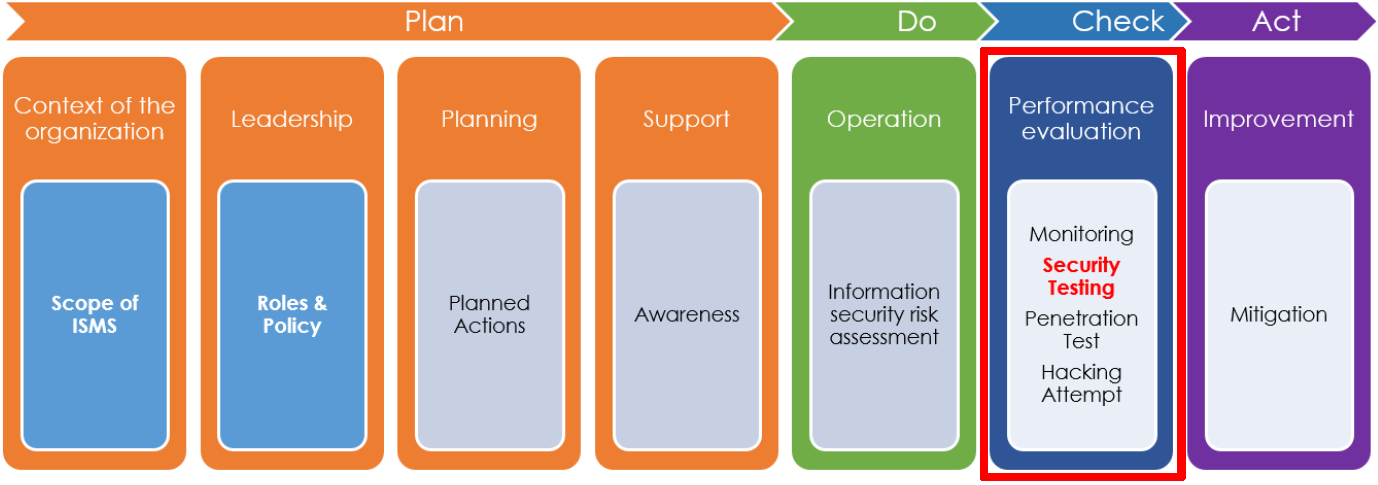
\includegraphics[width=\textwidth]{./img/ISO27001_overview}
	\caption{Stark vereinfachte Sicht [ISO27001:2005]}
\end{figure}

\begin{description}
	\item[Threat] Effekte, \textbf{können nicht} kontrolliert werden (Erdbeben, Stromausfall).
	\item[Risk] Risiko, kann vermindert werden durch verminderung des Einflusses auf das Business.
	\item[Vulnerability] Gefahren, können behandelt werden (Verbesserung der Software, Einschränken von Zugriff).
	\item[Vulnerability Assessment] Das eigentliche Information Security Management: Geschäftsprozesse werden beobachtet, verknüpft mit der Compliance, Budget, Beurteilung und der Bewusstheit der Gefahr.
	\item[Direct Attacks] Angriff direkt auf das Ziel, z.B. durch eine Firewall.
	\item[Indirect Attack] Ein ungeschütztes Gerät, wie z.B. ein privates Notebook, wird angegriffen und über dieses dann dem Angreifer Zugriff auf das restliche System ermöglicht.
	\item[Man-in-the-Middle] Der Angreifer hört den Datenverkehr des Opfers mit und kann diesen auch beeinflussen, erneut versenden oder verändern.
	\item[Privilege Escalation] Es wird versucht, mehr Berechtigungen zu erhalten, wie z.B. ausführen eines Skripts als Root, ohne die Kennwörter zu besitzen.
	\item[Social Engineering] Umgehen von technischen Einrichtungen zum Schutz vor Angriffen über menschliches Fehlverhalten und gezielte Manipulation des Menschen.
	\item[Backdoor] Teil einer Software/Hardware, unter Umgehung der normalen Zugriffssicherung Zugang zu geschützten Daten zu erlangen.
\end{description}

\subsubsection{Symantec Internet Security Threat Report}
Symantec veröffentlich seit nunmehr 20 Jahren jeden Frühling ihren Internet Security Threat Report, der jeweils die wichtigsten Bedrohungen des vergangenen Kalenderjahres analysiert und im Vergleich zu vorhergehenden Jahren die aktuellen Trends aufzeigt.

Folgende Punkte werden hauptsächlich thematisiert:
\begin{easylist}[itemize]
	& Mobile Devices
	& Internet of Things
	& Web Threats
	& Social Media, Scams and Email Threats
	& Targeted Attacks
	& Data Breaches
	& Cloud Infrastructure
	& Best Practice Guidelines
\end{easylist}

\section{Secure Software / Software Security}

Durch das Aufkommen des Internets nahm auch die vom \textit{National Institute of Standards and Technology} (NIST) erfassten Vulnerabilities mit hohem Ausmass zu.

\subsection{Most Dangerous Software Errors}
Die 25 häufigsten Schwachstellen können in drei Kategorien eingeteilt werden:
\begin{itemize}
	\item Ausgelöst durch unsichere Wege, in denen die Daten gesendet und empfangen werden. Dazu zählen \textit{SQL Injection}, \textit{OS Command Injection}, \textit{XSS}, \textit{CSRF} und \textit{Open Redirect}.
	\item Ausgelöst durch die unsichere Handhabung von Systemressourcen. Dazu gehören \textit{Classic Buffer Overflow}, \textit{Path Traversal}, \textit{Uncontrolled Format String}, \textit{Potentially Dangerous Function} und \textit{Integer Overflow}.
	\item Ausgelöst durch falsche Verwendung, Missbrauch oder Ignorierung von defensiven Sicherheitsmechanismen. Dazu zählen \textit{Missing Authentication}, \textit{Missing/Incorrect Authorization}, \textit{Hard-Coded Credentials}, \textit{Missing Encryption}, \textit{Reliance on Untrusted Inputs}, \textit{Incorrect Permission Assignment}, \textit{Use of broken or risky Cryptographic algorithm} und \textit{One-Way Hash without Salt}.
\end{itemize}

\subsection{Trinity of Trouble}
Folgende drei Aspekte sind mitunter verantwortlich für diese Schwierigkeiten.
\begin{description}
	\item[Connectivity] Immer mehr Systeme sind über das Internet miteinander verbunden und eröffnen somit neue \textit{Attack Vectors}. \textit{Service Oriented Architecture (SOA)} führt alte Systeme, welche nicht für die Vernetzung vorgesehen wurden, zusammen und veröffentlicht diese.
	\item[Extensibility] Systeme sind erweiterbar, wodurch ein teil der Kontrolle abgegeben wird. Über schlecht gewartete Erweiterungen können so neue Schwachstellen entstehen.
	\item[Complexity] Moderne Software wird immer komplexer. Mit dem Umfang nimmt auch die Fehlerrate quadratisch zu.
\end{description}

\subsection{Bugs + Flaws = Defects}
\begin{description}
	\item[Security Bug] Implementation-level Schwachstelle
	\item[Security Flaw] Design-level Schwachstelle (können selten automatisiert erkannt werden)
	\item[Security Defect] Ruhender defekt in der Software, welcher durch ein Bug oder Flaw ausgelöst wird.
\end{description}

\subsection{Software Artefakte}
Es gibt ein gemeinsames Set von Artefakten, welche unabhängig vom eigentlichen Entwicklungsprozess (Scrum, RUP, XP, \ldots) sind. Diese sind:
\begin{easylist}[itemize]
	& Anforderungen und Use Cases
	& Architektur und Design
	& Testpläne
	& Code
	& Tests und Testresultate
	& Rückmeldung von Kunden
\end{easylist}

\subsection{Drei Säulen der Software Security}

Zu den zentralen drei Säulen gehören \textbf{Risiko Management}, \textbf{Best Practices} und \textbf{Fachwissen}.

\subsubsection{Risiko Management}
Man identifiziert die betroffenen Personen, die technischen Risiken, auch die für das Unternehmen, und priorisiert sie anhand der gewonnenen Informationen. Danach kann eine Strategie zur Minderung entwickelt werden. Nach der Anwendung sollten die Anpassungen auf ihre Wirkung hin überprüft werden.

\begin{figure}[H]
	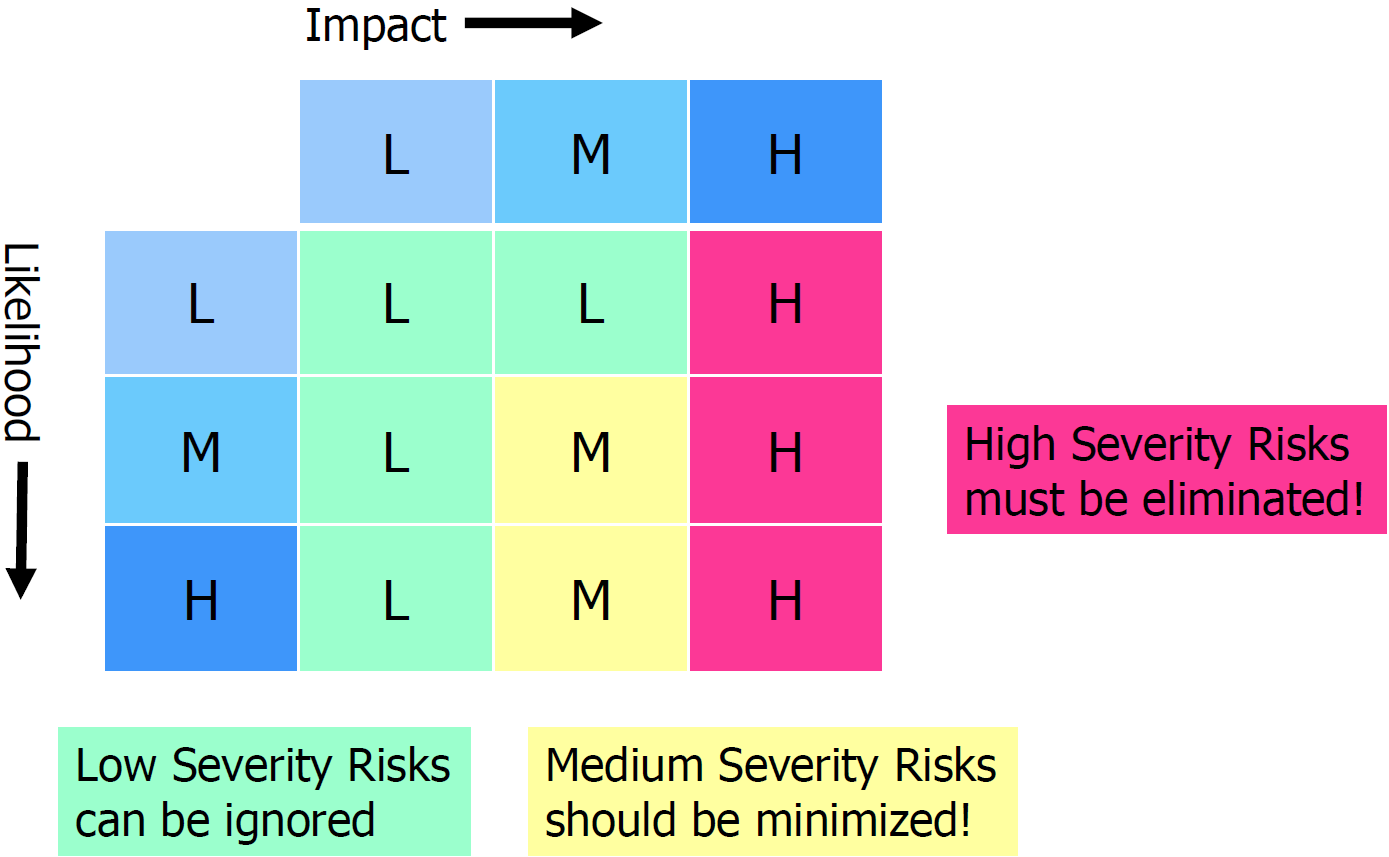
\includegraphics[width=0.6\textwidth]{./img/risk-evaluation}
	\caption{Risiko Evaluations-Matrix}
\end{figure}

\subsubsection{Best Practices}

Es folgen einige Best Practices in der Reihenfolge ihrer Effektivität. Sie können den Kategorien \textbf{K}onstruktiv (white hat) und \textbf{D}estruktiv (black hat) zugeordnet werden.
\begin{easylist}
	& Code Review \textbf{K}
	& Architectural risk analysis (historical knowledge) \textbf{K D}
	& Penetration testing \textbf{D}
	& Risk-based security tests \textbf{D K}
	& Abuse cases \textbf{D K}
	& Security requirements \textbf{K}
	& Security operation \textbf{K}
\end{easylist}

\subsubsection{Fachwissen}
Zum Fachwissen gibt es mehrere Perspektiven. Das Wissen über die Prinzipien, Rahmenbedingungen und Regeln gehören zum Vorgeschriebenen Fachwissen. Dazu gesellt sich die Diagnostischen Fähigkeiten mit dem Wissen über Angriffe, Schwachstellen und Angriffsmuster. Zuletzt benötigt man auch ein Wissen über die Vergangenheit.

\begin{figure}[H]
	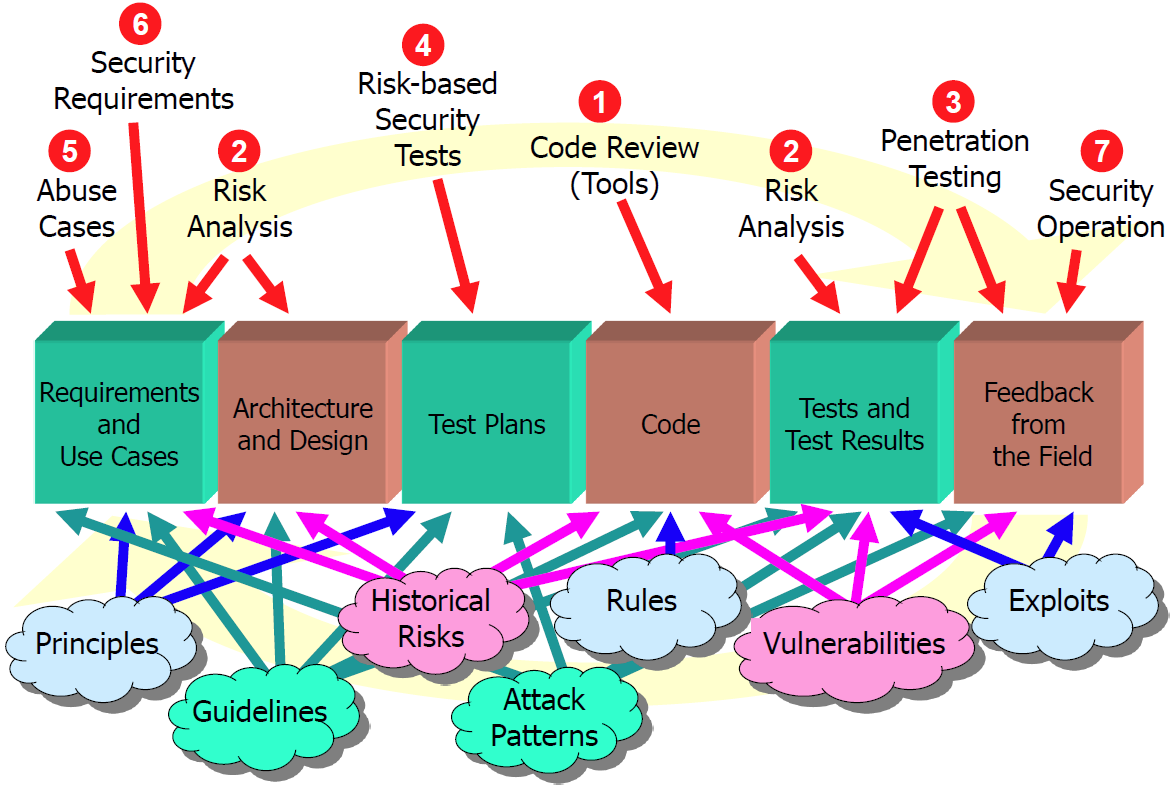
\includegraphics[width=\textwidth]{./img/sdl-best-practice}
	\caption{Best Practices und Fachwissen angewendet auf die Software Artefakte}
\end{figure}

\subsection{Code Analyse}

Für die Analyse von Sourcecode bieten sich mehrere Lösungen an, welche den Quellcode und auch das laufende Programm analysieren und auswerten können. Die ersten Generationen von solchen Analyseprogrammen wurden auch als \textit{Intelligentes Grep} bezeichnet und lieferten viele false positives. In späteren, oft kommerziellen Tools, wurden diese, durch Parsen des Source-Codes, versucht zu minimieren.

Das Wissen aus der Vergangenheit ist in die Regelsätze dieser Software eingeflossen. Jedoch können Probleme in der Softwarearchitektur nicht oder nur selten erkannt werden. Ein manuelles Review ist somit weiterhin nötig. Auch können Abhängigkeiten und falsche Benutzung externer Komponenten nicht korrekt überprüft und erkannt werden.

\subsection{Security Development Lifecycle - SDL}

Der Security Development Lifecycle ist ein Prozess, welcher die \textbf{Sicherheit innerhalb der Softwareentwicklung garantieren} soll. Er wurde von Microsoft entwickelt und gilt als Grundlage, lässt sich also für jede Unternehmensgrösse anpassen. Der SDL umfasst die drei Kernkonzepte \textbf{Schulung}, \textbf{fortwährende Verbesserung der Prozesse} und \textbf{Zurechenbarkeit}.\\
Der SDL sollte auf Projekte mit folgenden Merkmalen angewendet werden:
\begin{easylist}[itemize]
	& Eingesetzt in einem Unternehmen
	& Verarbeitung von personenbezogenen Daten
	& Regelmässige Kommunikation über das Internet oder andere Netzwerke
\end{easylist}
\textbf{Im Prinzip kann der SDL also auf alle Projekte angewendet werden.} Es ist einfacher, diejenigen zu identifizieren, die keinen sicherheitstechnischen Massnahmen benötigen und daher auch auf den SDL verzichten können.\\
Es existieren mehrere Rollen, wovon zwei besonders hervorzuheben sind. Diese lassen sich wiederum weiter unterteilen.
\begin{description}
	\item[Reviewer/Advisory Roles] Diese Rolle soll eine Übersicht über die Sicherheit des Projektes bieten und in der Lage sein, Pläne bezüglich Sicherheit und Datenschutz anzunehmen/abzulehnen. Kann von Internen wie auch externen Personen übernommen werden, aber keine Teammitglieder.
	\item[Team Champions] Diese Rolle ist verantwortlich für den Austausch, Akzeptanz und Verfolgung von minimalen Anforderungen an die Sicherheit und Datenschutz. Sie sind das Gegenstück zu den Advisory Roles und besteht aus Teammitglieder.
\end{description}

Finden die Sicherheitsrelevanten Aktivitäten frühzeitig und innerhalb des Entwicklungsprozesses statt, erhält man den grössten Nutzen daraus.
Um den Microsoft SDL-Prozess einzuhalten müssen die 16 zwingenden Aktivitäten eingehalten werden.

\begin{figure}[H]
	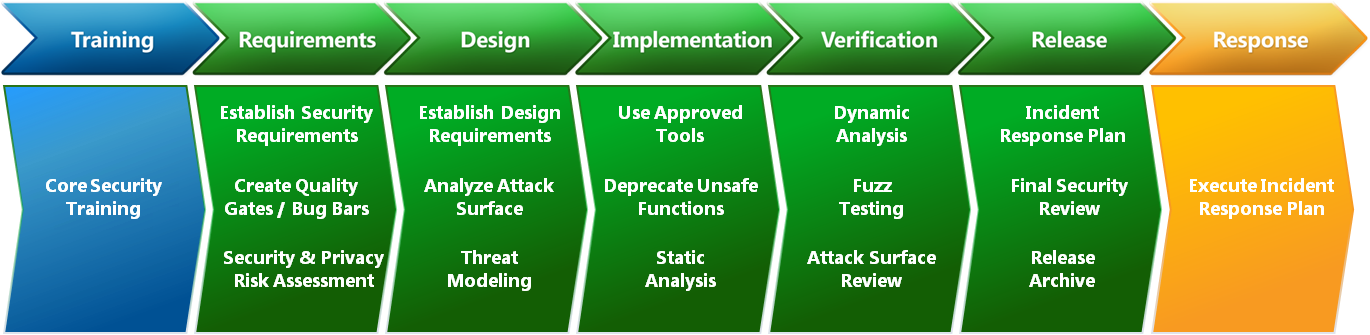
\includegraphics[width=\textwidth]{./img/sdl-overview}
	\caption{Security Development Lifecycle von Microsoft}
\end{figure}

\todo[inline]{Optionale Sicherheitsaktivitäten festlegen}

\subsubsection{Training Requirements}
Alle Mitglieder des Entwicklerteams müssen eine Schulung im Bereich Softwaresicherheit erhalten und sich über aktuelle Trends informieren. Die Themen umfassen \textbf{sicheres Design}, \textbf{Modellierung von Bedrohungen}, \textbf{sicheres Coding}, \textbf{Sicherheitstests} und \textbf{Datenschutz}.

\subsubsection{Security Requirements}
Definition von vertrauenswürdigen Anforderungen an das Projekt. Damit können Schlüsselstellen identifiziert werden und die Sicherheit sowie Datenschutz frühzeitig integriert werden. Dies verhindert unnötige Verzögerungen.

\subsubsection{Quality Gates/Bug Bars}
Quality Gates und Bug bars sind minimale Akzeptanzkriterien in Anbetracht der Sicherheit und des Datenschutzes. Das gesamte Team muss sich an die Anforderungen halten, wobei diese nicht dynamisch verändert werden dürfen.
\begin{description}
	\item[Quality Gate] Anforderung an die Code-Qualität bezüglich Compiler-Warnungen, Kommentare, Komplexität, etc.
	\item[Bug Bar] Schwelle für Sicherheitslücken, welche noch im Projekt beim Release enthalten sein dürfen. Z.B. keine Lücken mit der Bewertung "'Kritisch"' oder "'Warnung"'.
\end{description}

\subsubsection{Security and Privacy Risk Assesment}
Beurteilung der Sicherheit- und Datenschutz-Anforderungen von funktionalen Komponenten, welche eine genauere Begutachtung benötigen. Es wird bestimmt, ob weitere Threat Models, Security Design Reviews, Penetration Testing, Zusätzliche Tests und Anforderungen an Fuzz Tests nötig sind.\\
Zusätzlich wird das \textit{Privacy Impact Rating} festgelegt: \textbf{High Privacy Risk} bei der Verarbeitung von personenbezogenen Daten und Einstellungen, \textbf{Medium Privacy Risk} bei Übermittlung anonymisierter Daten und \textbf{Low Privacy Risk}, falls keine Anforderungen für den Datenschutz nötig sind.


\subsubsection{Design Requirements}
Designspezifikationen sollen Sicherheits- und Datenschutz-Funktionen beschreiben, welche direkt dem Benutzer zugänglich sind. Das sind z.B. Funktionen, welche eine Authentisierung oder die Einwilligung des Benutzers erfordern. Gleichzeitig sollten sie auch beschreiben, wie die Sicherheit dieser Funktion implementiert wird.

\subsubsection{Attack Surface Reduction}
Hierbei wird der Zugriff auf das System eingeschränkt und mehrschichtige Abwehrmassnahmen eingeführt. Eng verknüpft mit dem \textit{Threat Modeling}.

\subsubsection{Threat Modeling}
Es werden mögliche Bedrohungen in Betracht gezogen, Diskutiert und Dokumentiert im Kontext der geplanten Umgebung.

\subsubsection{Use Approved Tools}
Im gesamten Team müssen Tools definiert und festgehalten werden, wie damit die Sicherheit überprüft werden. Wie z.B. Compiler- oder Linter-Warnungen.

\subsubsection{Deprecate Unsafe Functions}
Als Team werden die Funktionen und APIs definiert, welche man nicht verwenden darf. Somit können diese dann auch überprüft und durch alternativen ersetzt werden.

\subsubsection{Static Analysis}
Eine skalierbare Möglichkeit zur Analyse des Codes auf Programmierfehler und Einhaltung der Coding-Guidelines. Dies schliesst aber manuelle Reviews nicht aus, diese sollten weiterhin für kritische Bereiche durchgeführt werden.

\subsubsection{Dynamic Program Analysis}
Verifikation während der Laufzeit, dass das Programm auch den Anforderungen entsprechend funktioniert. Es müssen Tools definiert werden, welche ein Fehlverhalten(falsche Berechtigungen) oder die Verwendung von Ressourcen protokollieren.

\subsubsection{Fuzz Testing}
Dynamische Analyse anhand von automatisch generierten Eingaben (absichtlich falsch oder zufällig). Die Strategie fürs Testen wird anhand der Funktionellen- sowie  Design-Spezifikation abgeleitet.

\subsubsection{Threat Model and Attack Surface Review}
Abweichungen der Anwendung von der ursprünglichen Funktionellen- und Design-Spezifikation feststellen und überprüfen, ob Anpassungen nötig sind. Spätestens beim Code-Complete ist eine erneute Analyse notwendig.

\subsubsection{Incident Response Plan}
Damit wird festgehalten, wie bei einem Notfall vorgegangen wird. Zudem sind weitere Informationen enthalten, welche für die Behebung und Verarbeitung hilfreich sind.
\begin{itemize}
	\item Ansprechperson für den ersten Kontakt sowie, wenn vorhanden, auch ein Entwicklerteam.
	\item Ansprechperson mit Entscheidungsgewalt, verfügbar 24/7.
	\item Sicherheitsrelevante Informationen von Code anderer Entwickler-Teams.
	\item Sicherheitsrelevante Informationen von Third-Party-Komponenten, dessen Version, Dateinamen, Kontaktdaten und Vertragsinformationen, falls vorhanden.
\end{itemize}

\subsubsection{Final Security Review}
Die eigentliche Kontrolle vor dem Release, ob die Software allen im Prozess definierten Anforderungen entspricht und die Sicherheitsaktivitäten eingehalten wurden. Hier werden die Gesammelten Informationen aus Threat Models, exception requests, Ausgabe der Tools und Performanz mit den Quality Gates und Bug Bar verglichen. Daraus ergibt sich dann das Resultat \textbf{FSR bestanden}, \textbf{FSR bestanden mit Ausnahmen} oder \textbf{FSR mit Eskalation}.

\subsubsection{Release/Archive}
Die Software ist aus Sicht des SDL komplett und kann nach Bestätigung des Sicherheitsberaters freigegeben werden. Für jede High Privacy Risk wird auch eine Bestätigung des Datenschutzbeauftragten benötigt.
Alle im Prozess erzeugten Artefakte müssen archiviert werden, um eine Wartung nach dem Release zu ermöglichen.

\section{Application Security Basics}


\todo[inline]{HTTP}
\todo[inline]{Cookies}
\todo[inline]{Session Handling}
\todo[inline]{Same Origin Policy}

\section{OWASP Top 10}
Die OWASP Top 10 sind die zehn kritischsten Schwachstellen von Web Anwendungen, welche aus dem \textit{Open Web Application Security Project} hervor gehen.\\

Die aktuellste Version ist 2013 in \fnurl{http://owasptop10.googlecode.com/files/OWASP\%20Top\%2010\%20-\%202013.pdf}{Englisch} erschienen und in mehrere Sprachen übersetzt, unter anderem auch \fnurl{https://www.owasp.org/images/4/42/OWASP_Top_10_2013_DE_Version_1_0.pdf}{Deutsch}. Die hier aufgeführten Kurzbeschreibungen stammen ebenfalls aus der deutschen Version.

\subsection{Injection}
Injection-Schwachstellen (SQL-, OS- oder LDAP-Injection) treten auf, wenn nicht vertrauenswürdige Daten als Teil eines Kommandos oder einer Abfrage von einem Interpreter verarbeitet werden. Ein Angreifer kann Eingabedaten dann so manipulieren, dass er nicht vorgesehene Kommandos ausführen oder unautorisiert auf Daten zugreifen kann.

\subsection{Broken Authentication and Session management}
Anwendungsfunktionen, die die Authentifizierung und das Session-Management umsetzen, werden oft nicht korrekt implementiert. Dies erlaubt es Angreifern Passwörter oder Session-Token zu kompromittieren oder die Schwachstellen so auszunutzen, dass sie die Identität anderer Benutzer annehmen können.

\subsection{Cross-Site-Scripting - XSS}
XSS-Schwachstellen treten auf, wenn eine Anwendung nicht vertrauenswürdige Daten entgegennimmt und ohne entsprechende Validierung oder Maskierung (\textit{escaping}) an einen Webbrowser sendet. XSS erlaubt es einem Angreifer Scriptcode im Browser eines Opfers auszuführen und somit Benutzersitzungen zu übernehmen, Seiteninhalte zu verändern oder den Benutzer auf bösartige Seiten umzuleiten.

\subsection{Insecure Direct Object References}
Unsichere direkte Objektreferenzen treten auf, wenn Entwickler Referenzen zu internen Implementierungsobjekten, wie Dateien, Ordner oder Datenbankschlüssel von aussen zugänglich machen. Ohne Zugriffskontrolle oder anderen Schutz können Angreifer diese Referenzen manipulieren, um unautorisierten Zugriff auf Daten zu erlangen.

\subsection{Security Misconfiguration}
Sicherheit erfordert die Festlegung und Umsetzung einer sicheren Konfiguration für Anwendungen, Frameworks, Applikations-, Web- und Datenbankserver sowie deren Plattformen. Sicherheitseinstellungen müssen definiert, umgesetzt und gewartet werden. Die Voreinstellungen sind oft unsicher. Des Weiteren umfasst dies auch die regelmässige Aktualisierung aller Software.

\subsection{Sensitive Data Exposure}
Viele Anwendungen schützen sensible Daten, wie Kreditkartendaten oder Zugangsinformationen nicht ausreichend. Angreifer können solche nicht angemessen geschützten Daten auslesen oder modifizieren und mit ihnen weitere Straftaten, wie beispielsweise Kreditkartenbetrug oder Identitätsdiebstahl begehen. Vertrauliche Daten benötigen zusätzlichen Schutz, wie z.B. Verschlüsselung während der Speicherung oder Übertragung sowie besondere Vorkehrungen beim Datenaustausch mit dem Browser.

\subsection{Missing Function Level Access Control}
Die meisten betroffenen Anwendungen realisieren Zugriffsberechtigungen nur durch das Anzeigen oder Ausblenden von Funktionen in der Benutzeroberfläche. Allerdings muss auch beim direkten Zugriff auf eine geschützte Funktion eine Prüfung der Zugriffsberechtigung auf dem Server stattfinden, ansonsten können Angreifer durch gezieltes Manipulieren von Anfragen ohne Autorisierung trotzdem auf diese zugreifen.

\subsection{Cross-Site Request Forgery - CSRF / XSRF}
Ein CSRF-Angriff bringt den Browser eines angemeldeten Benutzers dazu, einen manipulierten HTTP-Request an die verwundbare Anwendung zu senden. Session Cookies und andere Authentifizierungsinformationen werden dabei automatisch vom Browser mitgesendet. Dies erlaubt es dem Angreifer Aktionen innerhalb der betroffen Anwendungen im Namen und Kontext des angegriffen Benutzers auszuführen.\\
Gegenmassnahme: Form mit hidden field, das ein zufällig generiertes Token enthält und bei jedem Request serverseitig geprüft werden muss.

\subsection{Using Components with Known Vulnerabilities}
Komponenten, wie z.B. Bibliotheken, Frameworks oder andere Softwaremodule werden meistens mit vollen Berechtigungen ausgeführt. Wenn eine verwundbare Komponente ausgenutzt wird, kann ein solcher Angriff zu schwerwiegendem Datenverlust oder bis zu einer Serverübernahme führen. Applikationen, die Komponenten mit bekannten Schwachstellen einsetzen, können Schutzmassnahmen unterlaufen und so zahlreiche Angriffe und Auswirkungen ermöglichen.

\subsection{Unvalidated Redirects and Forwards}
Viele Anwendungen leiten Benutzer auf andere Seiten oder Anwendungen um oder weiter. Dabei werden für die Bestimmung des Ziels oft nicht vertrauenswürdige Daten verwendet. Ohne eine entsprechende Prüfung können Angreifer ihre Opfer auf Phishing-Seiten oder Seiten mit Schadcode um- oder weiterleiten.

\section{Identity and Access Management}

Unter \textbf{Federated Identity Management} gehören Abkommen, Standards und Technologien, um Identitäten und Berechtigungen über autonome Identitätsdomänen zu vereinheitlichen. Die \textit{Föderation} (Zusammenschluss) ermöglicht es, die Identitätsinformationen von verschiedenen Systemen transparent und sicher auszutauschen, um damit auf der Sicherheitsebene zusammenarbeiten zu können.\\

Logindaten und Identitäten sind also nur an einem Ort, dem \textit{Authentity-Provider}, gespeichert und dort findet auch jede Authentifizierung statt. Möchte nun ein fremdes System die Identität prüfen, so wird die Anfrage an den entsprechenden Authentity-Provider weitergeleitet und dessen Antwort abgewartet. Jeder Benutzer kann so einen eigenen Authentity-Provider haben.

\subsection[AAI]{Authentication \& Authorization Infrastructure - AAI}
\textbf{Ohne eine einheitliche AAI} benötigt jede zu schützende Ressource eine separate Benutzer-Administration und -Authentifikation. Probleme / Nachteile ohne AAI:
\begin{easylist}
	& Aufwändige und fehleranfällige Registrierung für jede einzelne Ressource
	& Unzuverlässige und veraltete Daten
	& Verschiedene Login-Prozeduren und Passwörter
	& Gewisse Ressourcen werden gar nicht erst benötigt
	& Ressourcen sind oft nur durch IP-Adressen geschützt
\end{easylist}

\textbf{Mit einer AAI} muss sich der Benutzer nur noch an einer Stelle authentifizieren. Diese kann dann an den verschiedenen Ressourcen für die Autorisierung verwendet werden. Vorteile durch AAI:
\begin{easylist}
	& Keine Registrierung pro Ressource nötig
	& Einheitliche Login-Prozedur
	& Neue Ressourcen können leicht hinzugefügt werden
	& Standortunabhängig
	& Weniger Kennwörter zu merken
\end{easylist}

\begin{figure}[H]
	\centering
	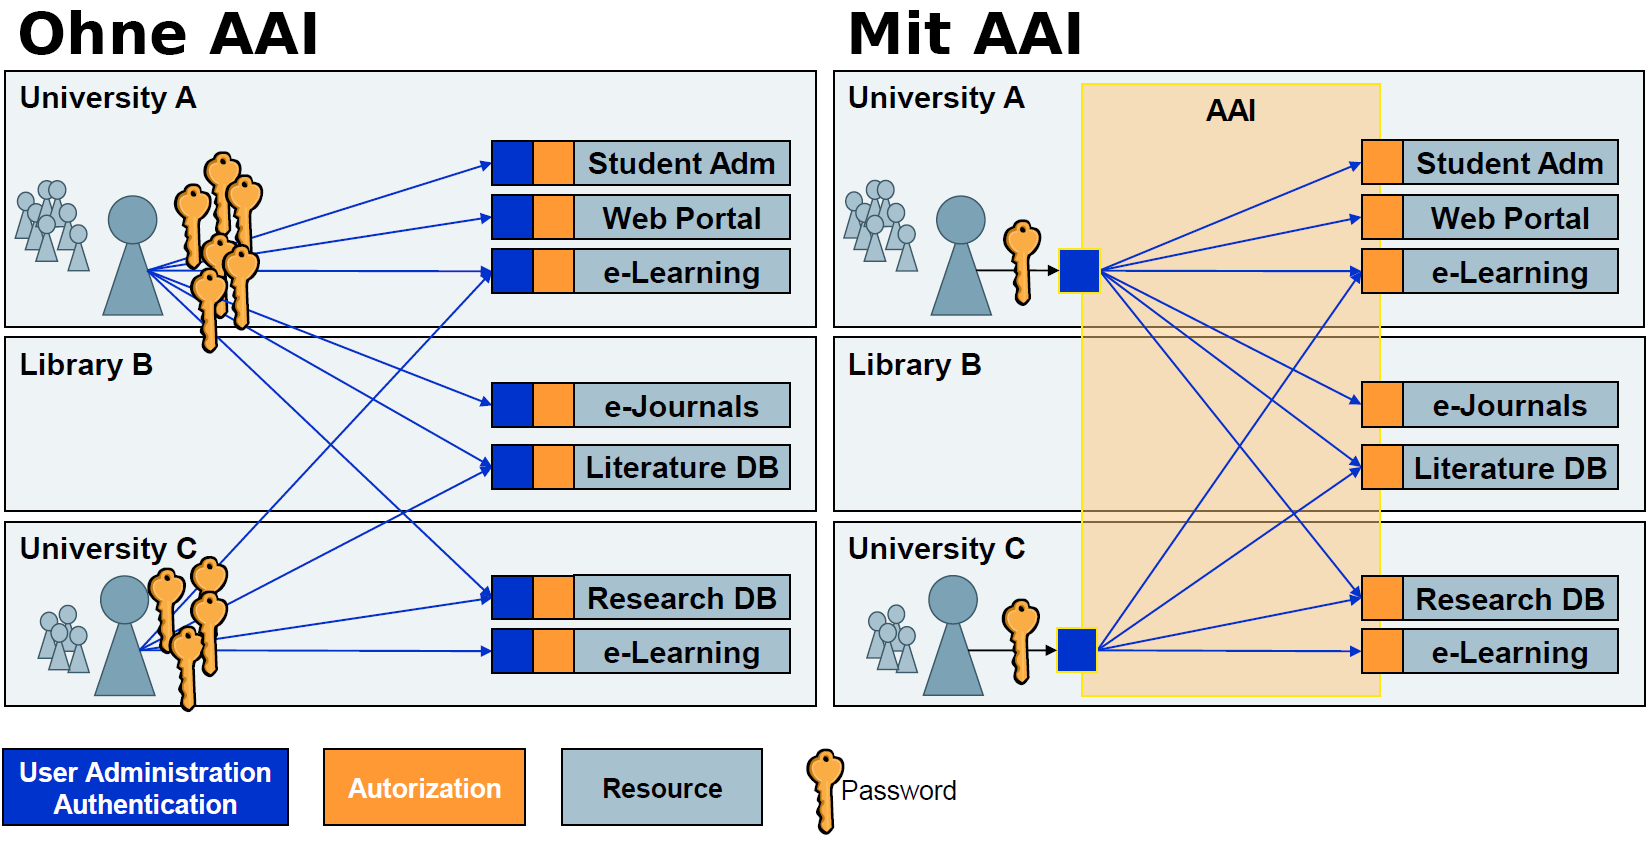
\includegraphics[width=\textwidth]{./img/AAI-example}
	\caption{Exemplarische Übersicht von AAI (Source: switch.ch/aai)}
\end{figure}

\subsubsection{Shibboleth}
Eines der weit verbreitetsten AAI, welches die Authentifizierung von Classic Web-Services über die Protokolle \textbf{SOAP, XML und SAML} übernimmt unter Verwendung von \textbf{http}.\\
Basiert auf \textbf{SAML-Assertions} (\textit{Security Assertion Markup Language}) ausgestellt von vertrauten Home-Organisationen (\textbf{Identity Providers}), welche von Ressourcen (\textbf{Service Providers}) aus dem Verbund akzeptiert werden.

\begin{figure}[H]
	\centering
	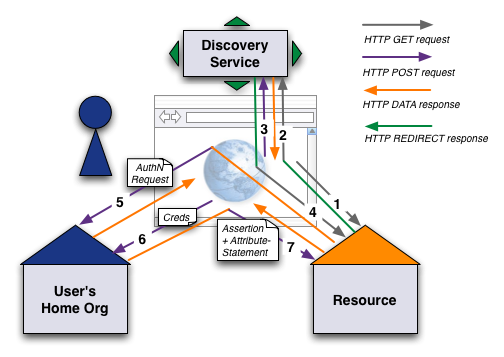
\includegraphics[width=0.7\textwidth]{./img/shibboleth-login}
	\caption{Vollständige Login-Prozedur mit Shibboleth (Source: switch.ch/aai)}
\end{figure}

\textbf{Beispiel}\\
Ein Beispiel für AAI mittels Shibboleth ist das System von SWITCH für Universitäten, mit dem man sich z.B. bei Unterrichtsplattformen oder Online-Shops mit dem Login seiner Uni- / Fachhochschule anmelden kann.\\
Dieses System übermittelt zudem \textbf{zusätzliche Attribute} zum authentifizierten Benutzer, wie etwa seine Mail-Adresse oder SwissEduPersonUniqueID.\\

\textbf{Standards}\\
Der Standard \textbf{XML Signature Syntax and Processing} erlaubt die Signierung, Integritätsprüfung und Nachrichtenauthentifizierung.\\
Der Standard \textbf{XML Encryption Syntax and Processing} erlaubt die Verschlüsselung von Daten innerhalb eines XML-Dokuments.\\
Der Standard \textbf{Secure Assertion Markup Language 2.0} kombiniert \textit{XML Signature Syntax} und \textit{XML Encryption Syntax} in einem Dokument mit Authentifizierung, Attributen und Autorisierung. Das resultierende XML-Dokument ist eine portable Identität für \textbf{Single Sign-On Web Services}.\\
Die Verwendung von SAML bringt als Vorteil mit sich, dass bestehende Enterprise-Anwendungen direkt integriert werden können. Das zugrunde liegende XML bringt aber dennoch etwa \textbf{90\% Overhead} mit sich.\\

Über die Architektur von \textbf{SuisseID} lässt sich so z.B. auch die \textbf{Alters-Verifikation} sicherstellen, da für die Ausstellung eine Identitätsprüfung durchgeführt wird.

\subsubsection{OAuth2}
OAuth2 wurde für neuere Protokolle wie \textbf{REST und JSON} entworfen und kommuniziert über \textbf{https}. Es gibt keine eingebauten Verschlüsselungs-Algorithmen, sondern es wird komplett auf TLS (https) vertraut. Die Funktionsweise ist \textbf{vergleichbar mit Kerberos}.

\begin{description}
	\item[Resource Owner] Benutzer
	\item[Resource Server] Die API
	\item[Authorization Server] Autorisiert den Benutzer (ist oft auf dem selben Server wie \textit{Resource Server})
	\item[Client] Thirt-Party Applikation, welche auf die API zugreifen möchte.
\end{description}

\begin{figure}[H]
	\centering
	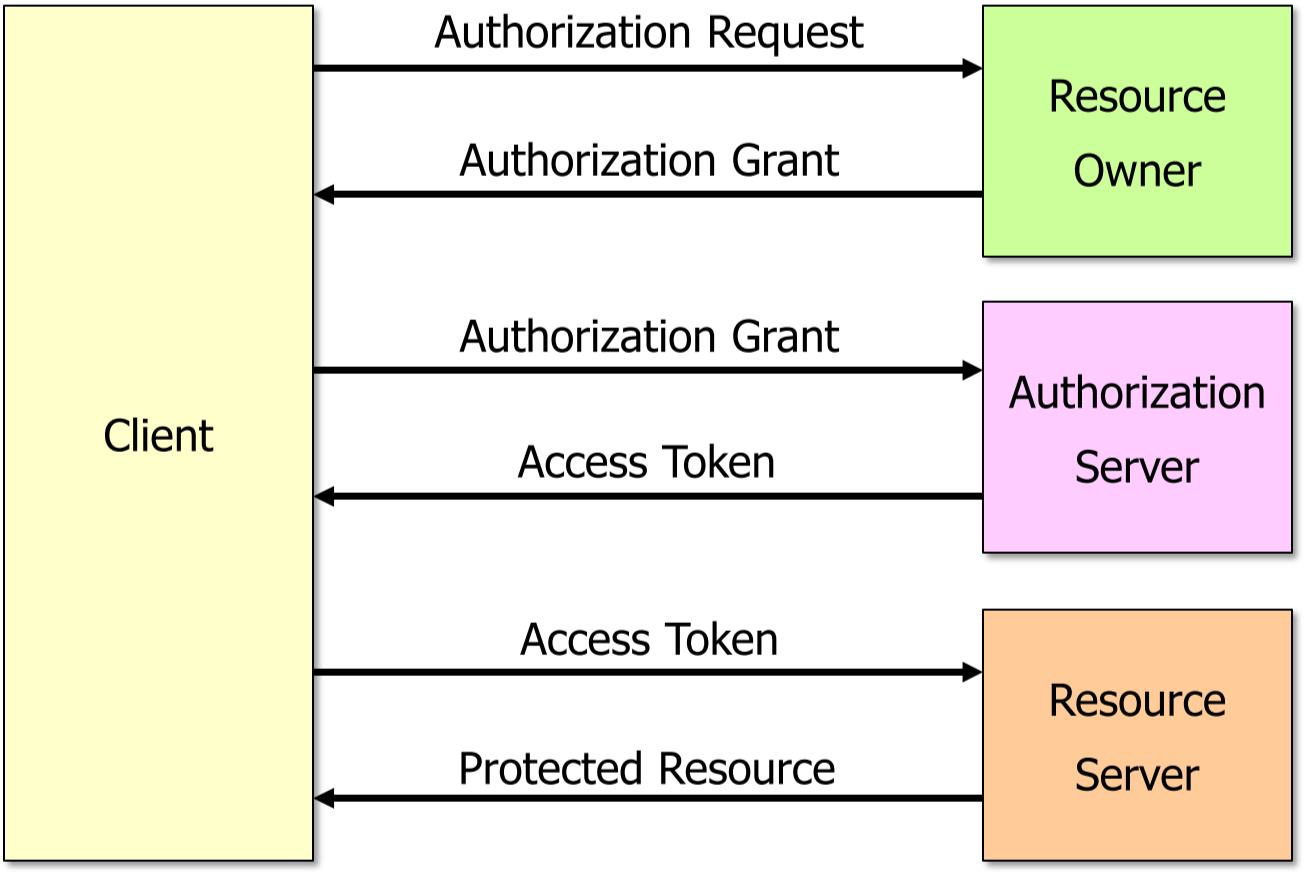
\includegraphics[width=0.5\textwidth]{./img/oauth2-example}
	\caption{Beispiel eines Zugriffs auf geschützte Ressourcen mittels OAuth2}
\end{figure}

Man kann OAuth2 nicht als zuverlässige Benutzerauthentifizierung zählen. \textit{OpenID connect} versucht dieses Problem zu lösen.\\

Jeder Anbieter setzt eine andere Version davon ein oder sogar eine eigene Implementierung.

\subsubsection{OpenID Connect}
\begin{easylist}[itemize]
	& OpenID Connect 1.0 is a simple identity layer on top of OAuth 2.0.
	& OpenID Connect 1.0 specifies a REST-based http API, using JSON as a data format..
	& OpenID Connect 1.0 uses a JSON Web Token (JWT) which can be signed using JSON Web Signature (JWS) and optionally encrypted using JSON Web Encryption (JWE).
	& OpenID Connect 1.0 is used by Google+ Sign-In.
\end{easylist}

\section{Web Entry Server}
Ohne Massnahmen werden mehrere Verbindungen direkt zu den Applikationsserver in der DMZ gemacht. Um dies zu verhindern wird eine \textbf{Web Application Firewall}(WAF) eingesetzt. Diese kann folgende Funktionen übernehmen:
\begin{easylist}[itemize]
	& Network Filter Level
	& SSL Termination
	& Protocol Validation and Rebuilding
	& Character Encoding and Unicode Verficatoin
	& White/Black List Filter
	& Cookie Protection
	& URL Encrypting
	& Smart Form Protection
	& Response Content Filter
	& Response Rewriting
\end{easylist}

\subsection{Reverse Proxy}
\todo[inline]{Reverse Proxy}
\subsection{Pre-Authentication}
Der Zweck einer Pre-Authentication ist dass jegliche \textbf{Backend Requests} bereits \textbf{authentifiziert} sind. Zudem werden \textbf{forensische und Log-Daten} abgelegt für spätere Verwendung.
\subsection{Filtering}
\todo[inline]{Filtering}
\subsection{Unique ID}
\todo[inline]{Unique ID}
\subsection{Smart Filtering und URL Encryption}
\todo[inline]{Smart Filtering und URL Encryption}

\section{Server Secuirty}

Man sollte davon ausgehen, dass die verwendete Software Schwachstellen besitzt. Auch wenn diese Schwachstellen nicht ausreichen, können sie dennoch als Sprungbrett für andere Angriffe verwendet werden. Daher ist es zwingend Nötig, das System auf allen möglichen Ebenen zu Härten und damit die Sicherheit zu erhöhen. Man spricht dabei von einer \textbf{Multi-Defense Strategy}.\\

Statistisch gesehen existiert für eine neu entdeckte Sicherheitslücke nach \textbf{6 Tagen ein Exploit} und erst \textbf{nach 54 Tagen ein Patch}. Oftmals ist Lesezugriff ausreichend, um einem Unternehmen Schaden zuzufügen oder daraus zu profitieren. Schreibzugriffe sind ebenfalls nicht zu vernachlässigen.\\

Besitzt der Angreifer Schreibzugriff, so kann er Anwendungen auf den Server laden und diese später ausführen. Beispiel: PHP Shell.

\subsection{Hardening}

\subsubsection{Während der Installation des Systems}
\begin{easylist}[itemize]
	& Minimales System
	& Keine Standard-Pfade
	& Separate Disk/Partition für log files
	& Aktuellste Patches eingespielt
	& Default Secure (Umask, Path)
	& Verwendung eines Install Servers
\end{easylist}

\subsubsection{Netzwerksicherheit}
\begin{easylist}[itemize]
	& Nur benötigte Dienste starten
	& Least File Permissions für Dienste anwenden
	& Least Process Privileges anwenden
	& Standard-/Beispielinstallationen entfernen
	& Banner Hiding (keine Versionsinformationen sichtbar)
	& Error Handling (keine Fehlerdetails sichtbar nach aussen)
\end{easylist}
\subsubsection{Authentifizierung}
\begin{easylist}[itemize]
	& Verwendung einer sicheren Authentifizierung (Benutzername, Kennwort, OTP, Client Certificate)
	& Password Policy (Stärke, Gültigkeitsdauer, Kennwortwechsel, Erkennung von Attacken auf geknackte Passwörter)
\end{easylist}
\subsubsection{Monitoring und Auditing}
\begin{easylist}[itemize]
	& Zeitsynchronisation
	& Integritätstests
	& Event handling (info, debug, error, panic, log)
	& Forensic Readiness
	& Remote Logging
\end{easylist}

\subsection{Unix Process Security}
Unter Linux ist ein weit verbreiteter Ansatz in der Prozess-Sicherheit die \textbf{Isolierung durch Chroot} (change root). Dabei wird dem Prozess ein angegebenes Verzeichnis als Root vorgegaukelt. Innerhalb des neuen Root-Verzeichnis befinden sich alle für den Service nötigen Dateien. Er kann dabei nicht auf Dateien zugreifen, welche sich ausserhalb des neuen Root-Directories besitzen. Man spricht dabei auch von einem Jail.\\

Durch Schwachstellen im Unix-Kernel ist es aber trotzdem möglich, aus diesem Jail auszubrechen.

\subsection{File Permissions}
Die Berechtigungen auf Dateisystemebene sollten so restriktiv wie möglich sein. Als Grundsatz gilt: \textbf{Never give "'world"' write access}. Dasselbe gilt für sensitive Informationen: \textbf{Keep sensitive data secure by removing read access from "'world"'}.\\

Um die Standard-Berechtigungen unter Unix zu setzen, kann mit einer Maske gearbeitet werden. Diese ist auch bekannt als "'Umask"'. Um die obigen Berechtigungen für den aktuellen Prozess zu ändern, kann z.B. \lstinline|$ umask 027|.\\

Durch dieses Vorgehen kann auch die Gefahr einer \textbf{Local File Inclusion} vermindert werden.

\begin{figure}[H]
	\centering
	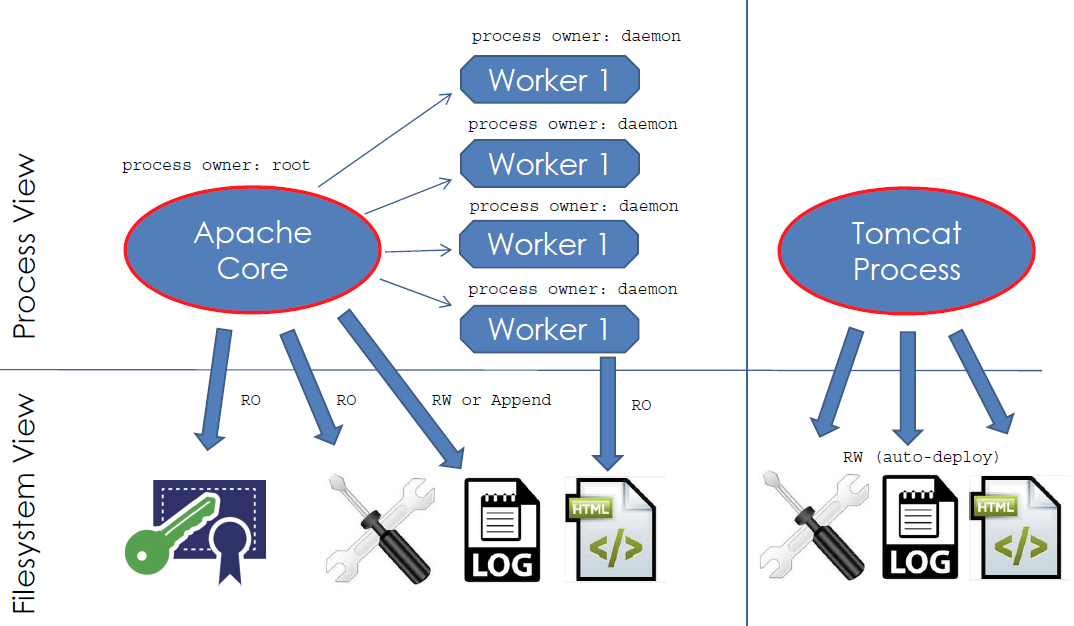
\includegraphics[width=\textwidth]{./img/apache_tomcat_permissions}
	\caption{Beispiel der Berechtigungen für Apache und Tomcat}
\end{figure}

\subsubsection{Apache File Permissions}
\begin{easylist}[itemize]
	& Im Besitz von Root
	&& Konfigurationsdateien
	&& SSL Schlüssel
	&& Log
	&& Html
	& Eigentümer des Apache Prozess benötigt nur RO
	&& Html
\end{easylist}

\subsubsection{Tomcat File Permissions}
Dies gestaltet sich oftmals schwierig, denn Tomcat besitzt eine andere Prozess-Architektur. Der Eigentümer des Tomcat-Prozess benötigt RW, für Remote Deployment, Konfiguration und Load Balancing.

\subsection{Privilege Escalation}
Dabei versteht man die Möglichkeit, die Berechtigungen des aktuellen Prozesses so zu verändern, dass man Zugriff auf andere geschützte Elemente erhält. Dazu können z.B. Bugs in SetUID-Tools verwendet werden.\\

Aber auch CRON kann gefährlich sein, da die Prozesse als Root gestartet werden. Wenn nun ein von CRON-Skript "'world-writeable"' ist, kann somit schnell etwas mit höchsten Berechtigungen ausgeführt werden.

\subsection{Network Hardening}
\textbf{Nur die nötigsten Dienste} sollten gegen Anfragen von aussen reagieren. Alle anderen müssen an \textit{localhost} gebunden sein. Alternativ kann auch eine \textbf{Firewall} dafür eingesetzt werden.\\
Dienste wie UPNP, Bonjour / Zeroconf und DLNA sollten aufgrund ihrer grossen Attach-Surface auch deaktiviert werden. Dies stammt daher, dass oftmals die Geräte unzureichende Authentifizierungsmechanismen implementiert haben.\\

Es wird in den Folien auch von der \textbf{Verwendung von IPv6 abgeraten}.\\

\textbf{ICMP-Redirects deaktivieren}, um MITM-Attacken vorzubeugen.\\

Eine Analyse mittels Nmap oder \fnurl{https://cisofy.com/lynis/}{Lynis von Cisofy} helfen, Schwachstellen aufzudecken.

\subsection{DB Hardening}
Wie auf das Dateisystem trifft das Prinzip Least Privileges auch auf die Datenbank zu. Der in der Anwendung hinterlegte Benutzer darf nur auf seine Datenbanken Berechtigungen erhalten. Es können in einer Anwendung auch mehrere Benutzer hinterlegt werden, mit unterschiedlichen Berechtigungen. So z.B. ein Benutzer nur mit \textit{SELECT}-Permissions für Abfragen, \textit{INSERT} und \textit{UPDATE} für Bestellungen und ein \textit{CREATE}, \textit{DELETE} für den DB-Admin.\\
\textbf{Keinesfalls sollte der Applikations-User \textit{GRANT}-Permissions erhalten.}

\section{Mobile Application Security}

\subsection{iOS}
Basierend auf OSX hat Apple das iOS lanciert. Dabei wurde Objective-C, Swift, und C verwendet. iOS verfügt über Sandbox Mechanismen, ein Data Protection API, Code Signing und den Appstore mit manueller Freischaltung.

\begin{figure}[H]
	\centering
	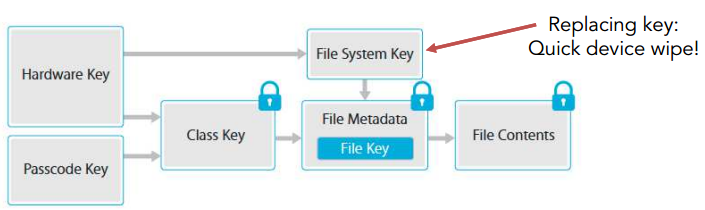
\includegraphics[width=0.6\textwidth]{./img/mobileappsecurity_iOS-DataProtectionAPI}
	\caption{iOS Data Protection API}
\end{figure}

Bei iOS ist das \textbf{Permission Model} so eingerichtet, dass bei jeder Verwendung nach Erlaubnis gefragt wird und individuell erlaubt oder abgelehnt werden kann.

\subsection{Android}
Auf Linux basierend in Java und C entstand Andoid, welches von verschiedene Hardware-Anbietern übernommen wurde. Somit hat es auch noch viele alte Versionen auf dem Markt.

Android unterstützt SD Karten, Sandboxing via JVMs, Code Signing, und mehrere verschiedene Appstores.

Die \textbf{App Permissions} sind bei Android im Manifest hinterlegt und können ab Android 6 individuell angenommen oder abgelehnt werden.

\subsection{Windows Phone}
Windows Phone von Microsoft unterstützt ebenfalls strict sandboxing, Address Space Layout Randomization (ASLR, zufällige Ladeposition von Programmen in Speicher als Schutz gegen Overflow), Bit Locker Verschlüsselung, Data Protection API (ähnlich wie bei iOS), aber auch Gefahren wie automatisches Wi-Fi credential sharing über Facebook, Outlook oder Skype. (In Version 1607 wurde die umstrittene Funktion \textit{Wi-Fi Sense} wieder entfernt.)

\subsection{Xamarin}
Xamarin ermöglicht die Entwicklung von platformübergreifenden, nativen Apps. Dabei wird das Mono Framework (.NET kompatibel) verwendet und in C\# programmiert, welches zu IL-Code (Microsoft Intermediate Language) kompiliert wird.

Die native APIs werden zwar zu den .NET namespaces gemapped, jedoch müssen platformabhängige Security Features sowie User Interfaces immer noch für jede Platform geschrieben werden.

\subsection{Cordova (Phonegap)}
Cordova wird verwendet um Mobile Apps mit HTML, JS und CSS zu entwickeln. Es bringt somit native Funktionalität, basiert aber auf Web View Komponente. Somit fallen jedoch auch alle bekannten Schwachstellen an.

\section{OWASP Mobile Top 10}
\begin{figure}[H]
	\centering
	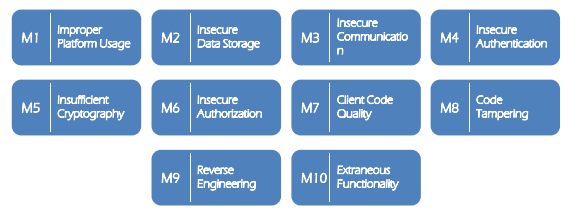
\includegraphics[width=0.8\textwidth]{./img/OWASP_MobileTop10}
	\caption{OWASP Mobile Top 10, 2016}
\end{figure}

\subsection{M1: Improper Platform Usage}
Missbrauch eines Platform Features oder fehlende Sicherheitsmassnahmen, und das somitige Verletzten von Guidelines. \\

\textbf{Beispiel}: Zu viele Permissions, unverschlüsseltes Ablegen von Credentials in Property-File anstelle der KeyChain (iOS). \\

\textbf{Lösung}: Konsultieren der Platform Guidelines beim Entwickeln.

\subsection{M2: Insecure Data Storage}
Durch Ablegen von Daten in unsicherem Speicher oder unvorhergesehenem Datenleak (siehe Unterkapitel) besteht erhöhte Gefahr wenn das Gerät gestohlen wird/verloren geht oder mit Malware infiziert ist nach jailbreak/rooting.

\subsubsection{System Screenshots}
Das Betriebssystem erstellt ein Screenshot der Anwendung, um diese unter den zuletzt verwendeten Anwendungen darzustellen. Manchmal aber auch in anderen Fällen.\\

\textbf{Beispiel}: E-Banking Kontoinformationen können eingesehen werden über den Screenshot des Apps. \\

\textbf{Lösung}: Screenshots vom System unterbinden oder sensitiven Daten überdecken.
\begin{lstlisting}[language=C, caption=Lösung für iOS]
(void) applicationDidEnterBackground:(UIApplication *)application{
	// mask the sensitive data or add an additional layer on top			
}
\end{lstlisting}
\begin{lstlisting}[language=Java, caption=Lösung für Android]
window.addFlags(LayoutParams.FLAG_SECURE, LayoutParams.FLAG_SECURE);
\end{lstlisting}

\subsubsection{Keyboard}
Viele Keyboards verfügen über Autocomplete. Das iOS zum Beispiel speichert bis zu 500 Wörter.\\

\textbf{Beispiel}: Passwort Feld unterstütz Autocomplete; Das Passwort wird somit auch an anderen Stellen vorgeschlagen wenn mit dem selben Buchstaben begonnen wird. \\

\textbf{Lösung}: Autocomplete bei sensitiven Daten deaktivieren.
\begin{lstlisting}[language=C, caption=Lösung für iOS]
theTextField.secureEntry = YES;
theTextField.autocorrectionType = UITextAutocorrectionTypeNo;
\end{lstlisting}
\begin{lstlisting}[language=Java, caption=Lösung für Android]
android:inputType="textNoSuggestions";
\end{lstlisting}

\subsubsection{Clipboard}
Standardmässig wird ein globales Clipboard für Copy \& Paste verwendet, und jedes App kann darauf zugreifen. \\
\textbf{Beispiel}: Sensitive Daten befinden sich noch im Clipboard aus der E-Banking App.

\textbf{Lösung}: Clipboard leeren oder ein dediziertes Clipboard verwenden.
\begin{lstlisting}[language=C, caption=Lösung für iOS]
UIPasteBoard *uniqueBoard=[UIPasteboard pasteboardWithUniqueName];
\end{lstlisting}

\subsubsection{Logs}
Crash- und Applikationslogs können sensitive Daten enthalten. Im Apple System Log (ASL) bei iOS werden sogar alle Logs gecached bis zum nächsten Reboot und auch nicht sandboxed. Bei Android müssen Debug Logs bei der finalen App deaktivieren werden. \\

\textbf{Beispiel}: Bei gescheitertem Loginversuch speichert das Log Benutzername und Passwort im Log. \\

\textbf{Lösung}: Dedizierter Logger für Debug Build der App.

\subsubsection{Web Data}
Eine WebView speichert jegliche Daten wie ein konventioneller Web Browser. Dies umfasst ein Web Cache, lokaler Speicher, Cookies, Passwörter die direkt oder in eine Sqlite Datenbank gespeichert werden. \\

\textbf{Beispiel}: Ablegen von unverschlüsselten Passwörtern und Benutzernamen in Sqlite Datenbank.\\

\textbf{Lösung}: Korrekte Systemspeicher verwenden.

\subsubsection{Inter-Process Communication}
Apps können URL Handlers registrieren, wobei der Empfänger und die überlieferten Informationen nicht geprüft werden können. Zudem entsteht ein Problem wenn mehrere Apps für ein Handler bestehen. Bei Android kann dann die aufzurufende Applikation gewählt werden, bei iOS wird die zuletzt installierte App automatisch ausgewählt.\\

\textbf{Beispiel}: Sensitive Daten werden bei Aufruf über einen Handler abgefangen.
\begin{lstlisting}[language=XML, caption=Aufruf von Skype]
skype://090012312312?call
\end{lstlisting}

\textbf{Lösung}: Bei Android direkter Aufruf eines Intent aus der anderen App.

\subsection{M3: Insecure Communication}
Das Verwenden von inkorrekten oder alten SSL Versionen, schwache Protokollaushandlung oder einfach Plain Text Kommunikation.

Ab iOS 9 wurde mit \textbf{App Transport Security} durch mimimum Anforderungen eingeführt (TLS 1.2 mit PFS, Zertifikat und SHA-256 Signatur, 2048-bit RSA oder 256-EC Key). Apps unterstehen diesen Vorbestimmungen oder müssen explizite Ausnahmen definieren.

\subsubsection{Certificate Pinning}
Standardmässig wird bestimmten Certificate Authorities (CA) vertraut. Deren Root Zertifikate sind auf jedem Gerät vorinstalliert.\\

\textbf{Beispiel}: Die CA wurde gehacked oder ein Attackierer hat dem Gerät eine falsche CA hinzugefügt. \\

\textbf{Lösung}: Certificate Pinning, eingeführt durch Google Chrome. Speichert das Zertifikat oder dessen Public Key in der App und überprüft dieses.

\subsection{M4: Insecure Authentication}
Das Verletzten von Privacy durch Mitschicken von Gerät-spezifischen Daten, spoofing, vohersehbare Session IDs, oder kein Session Timeout.

\subsection{M5: Insufficient Cryptography}
Schwache Ciphers und/oder Keys, ungeschützte Keys in App, oder sebstgemachte Bastel-Krypto.\\

Android besitzt die Bouncy Castle Library. Alternativ kann dieses auch in die App eingebunden werden als Klon, welches dann Spongycastle genannt wird.\\

iOS hat das Common Crypto API CCCRypt. Die KeyChain kann zudem für asymmetrische Kryptographie verwendet werden. Alternativ kann OpenSSL verwendet werden.

\subsection{M6: Insecure Authorization}
Das authorisieren von unerlaubten Benutzern oder Methoden ausführen von zu wenig authorisierten Benutzern. Ein klassisches Beispiel ist \textit{Forced Browsing}.

\subsection{M7: Client Code Quality}
Implementationsprobleme wie Buffer Overflows, XSS, format string Schwachstellen etc. Muss im Code selbst gefixed werden.

\subsection{M8: Code Tampering}
Es besteht die Möglichkeit dass Code selbst verändert oder ausgetauscht wird. Dazu gibt es mehrere Möglichkeiten:

\begin{description}
	\item[Binary/Monkey Patching] Runtime Patch ohne Kopie des originalen Source Codes.
	\item[Resource Modification] Manipulation von lokalen Ressource-Files, welche z.B. URLs beinhalten.
	\item[Method Hooking] Bei erweiterbaren Frameworks das missbrauchen von Hooks für eigene Zwecke.
	\item[Method Swizzling] Implementation zweier Methoden austauschen.
	\item[Jailbreak/Rooting] Root Access zu System, kann aber anhand von Filestrukturen, Libraries oder OS-abhängigen Merkmalen erkannt werden.
\end{description}

\subsection{M9: Reverse Engineering}
Der Code kann eingesehen werden durch Binary Inspection, Dissasembly oder geleaktem Source Code. Gegen die ersten zwei kann ein \textbf{Code Obfuscator} verwendet werden, wie etwa ProGuard im Android SDK. Grundsatz: Verlass dich nicht auf \textit{Security by Obscurity}.

\subsection{M10: Extraneous Functionality}
Schwachstellen wie Backdoors für die Entwickler, Funktionen die nicht für den Release gedacht wurden sondern lediglich für Tests, oder Passwörter in Kommentaren.

\subsection{Checkliste}
\begin{easylist}[itemize]
	& Data at Rest
	&& iOS: DataProtection && Keychain API
	&& Backup Exclusion
	&& Caching
	& Data in Motion
	&& Certificate Pinning
	&& Transport Security
	& Data Leakage
	&& Prevent side-channel leakage: logs, keyboard, screenshots...
	& Input Validation
	&& Input sanitization e.g. URL handler parameters
	&& Format strings
	& Code Protections
	&& Code Obfuscation
	&& Stack protection
	&& Anti-Debug controls
	&& Compiler settings
	&& Code Injection Checks
	& Web View Hardening
	&& Disable local file access
	&& Disable plugins
	&& Disable javascript	
	&& URL whitelisting
	& Environment integrity
	&& Jailbreak / Rooting detection
	&& Version control / mandatory updates
\end{easylist}



\section{Fraud Detection}
Fraud Detection beschreibt das Vorgehen um Betrugsfälle wie zum Beispiel beim E-Banking möglichst schnell zu erkennen und zu melden. Dabei wird der Computer als Hilfsmittel verwendet. Bis jetzt ist die Quote der gefundenen Fälle per Fraud Detection noch sehr gering. Weit über die Hälfte der Fälle werden durch Hinweise oder ein Management Review gefunden.
\subsection{Panopticlick / Client Correlator}
Panopticlick ist ein Softwareprojekt der Electronic Frontier Foundation (EFF). Die Idee der Software ist es aufzuzeigen dass ein Benutzer nur durch das Besuchen einer Website identifiziert werden kann, ohne dass man ein Passwort angeben muss. Dafür wird ein Javascript auf dem Client ausgeführt, welches Informationen über den Browser sammelt. Daraus wird eine CCID (Client Correlation ID) generiert. Diese wird auf dem Server mit bisherigen CCIDs verglichen. Somit kann man feststellen ob der Request von einem bereits bekannten Gerät kommt oder nicht. Um den Fingerprint des Browsers zu erstellen werden zum Beispiel folgende Daten analysiert:
\begin{easylist}[itemize]
	& Verschlüsselte IP
	& Installierte Fonts
	& Installierte Plugins
	& Screen Resolution
	& Name des OS
	& User Agent String
\end{easylist}
\subsection{E-Banking}
E-Banking Systeme Verwenden zwei unterscheidliche Informationstypen um allfällige Frauds zu erkennen.
Sollte bei der Überprüfung ein Verdacht auftauchen kann die Transaktion gesperrt oder zum Beispiel per Telefon vom User bestätigt werden.
\subsubsection{Technische Daten}
Die Technischen Daten werden aus der Session gelesen. Die ausgelesenen Daten werden gegen alte gesammelte Daten verglichen.
Unter Anderem werden folgende Daten verwendet:
\begin{easylist}[itemize]
	& User Agent
	& Source IP
	& Zeit
	& Tippgeschwindigkeit
	& Durchschnittliche eingeloggte Zeit
\end{easylist}
\subsubsection{Business Informationen}
Bei den Business Informationen geht es um die getätigte Transaktion selber. Aufgrund dieser Daten könnte eine Fraud Transaction eventuell erkannt werden.
folgende Punkte werden untersucht:
\begin{easylist}[itemize]
	& Betrag
	& erstmalige Zahlung
	& An welche Bank geht die Zahlung (Inland / Ausland)
\end{easylist}
\subsection{Data Mining}
Data Mining beschreibt den Vorgang um aus riesigen Mengen von Daten und Datensätzen die wichtigen Informationen und zusammenhänge herauszufiltern.
Diese Fähigkeit wichtige Informationen aus einer grossen Masse zu filtern ist besonders für Vorhersagen oder Machine Learning interessant.
Durch Data Mining werden die Daten in gruppen unterteilt.
Drei Common Tasks sind besonders nützlich für Fraud Detection:
\begin{easylist}[itemize]
	& Classification: Predictive, Kunden mit einer guten Kreditwürdigkeit suchen zum Beispiel
	& Clustering: Descriptive, Alle Kunden mit ähnlichem Einkaufsverhalten gruppieren
	& Association Rules: Artikel finden die oft mit dem gekauften zusammen gekauft werden
\end{easylist}
\subsection{Machine Learning}
Aufgrund der Informationen aus den Data Minings können Machine Learning Algorithmen eingesetzt werden, um zum Beispiel eine Transaktion als "Verdächtig" oder "Harmlos" einzustufen. Dies geschieht immer aufgrund bisher erhaltenen Transaktionen. Der Input (Neue Transaktion) wird also nacher als Richtwert für die nachfolgenden Transaktionen verwendet. So lernt der Automat dann von alleine. In der Vorlesung wurden verschiedene Algorithmen aufgezeigt:
\begin{easylist}[itemize]
	& Dempster–Shafer Theory
	& BLAST-SSAHA Hybridization
	& Hidden Markov Model
	& Evolutionary-fuzzy System
\end{easylist}

\section{Security Testing}

\subsection{Notwendigkeit}
Die Bedrohung von Informationssystemen ist allgegenwärtig und man kann jederzeit ein Ziel eines Angriffes werden. Auch aus der Sicht der Beteiligten gibt es viele verschiedene Risiken, welche als Treiber für ein Security Testing dienen.
\begin{table}[H]
	\begin{tabularx}{\textwidth}{l|X}
		\textbf{Rollen} & \textbf{Risiken}\\ \hline
		Firmeninhaber, -Teilhaber & Finanzielle Risiken, Verlust von Assets, Reputationsrisiko\\ \hline
		Aufsicht, Regulatoren & Schädigung des Wirtschaftsplatzes, Reputationsrisiko\\ \hline
		Verwaltung, Schulen & Druck der Aufsichtsbehörde\\ \hline
		Entwickler, Ingenieure, Forscher & Know-How Abfluss\\ \hline
		Sicherheitsverantwortliche & Jobverlust\\ \hline
		Kunden, Nutzer & Persönlichkeitsschutz (Datenschutz, Finanzielle Risiken)\\ \hline
	\end{tabularx}
	\caption{Risiko der Beteiligten in verschiedenen Rollen}
\end{table}

Bei einer Sicherheitsprüfung muss die Bedeutung aller Ebenen (Prozess-, Applikations- und Infrastruktur-Ebene) beurteilt werden. Es muss sichergestellt werden, dass der Prüfbereich sinnvoll (in Abhängigkeit der Risikoeinschätzung) festgelegt wird.

\todo[inline]{Ablauf}
\todo[inline]{Begriffe}

\section{Spezialthemen}


\subsection{XXE File Inclusion}
Unter dem Begriff ist eine Attacke über das \textit{XML External Entity Processing} möglich. Dabei können externe Daten, wie z.B. lokale Dateien, in das XML inkludiert werden. Bei der Verarbeitung solcher Inclusions, welche im DTD angegeben sind, fügt sie der Parser in die angegebenen Stelle ein.\\

\textbf{Lösung:} Deaktivierung des Features für DTDs (External Entities) beim Parser.

\begin{lstlisting}[language=XML, caption=Beispiel der XXE]
<?xml version="1.0" encoding="ISO-8859-1"?>
<!DOCTYPE foo [  
  <!ELEMENT foo ANY >
  <!ENTITY xxe SYSTEM "file:///etc/passwd" >]>
<foo>&xxe;</foo>
\end{lstlisting}

\subsection{JSON-Hijacking}
JSON-Hijacking zielt darauf ab, sensitive Daten, die mittels JSON Format an einen authentifizierten Empfänger übermittelt werden, zu stehlen. Dabei präpariert der Angreifer eine Seite mit einem JavaScript, welches die Callback-Funktion oder den \textit{Property Setter} überschreibt. Als zweites wird ein GET Request auf die verwundbare Seite durchgeführt. Die Response kann dann vom Angreifer verarbeitet werden und die Daten (möglicherweise sensitive Informationen) auf seinem System speichern.\\

\textbf{Lösung:}
\begin{easylist}
	& Token in Request URLs verwenden, sodass diese nicht erraten werden können
	& JSON Response mit einem Infinite Loop beginnen
	& JSONP vermeiden
	& Arrays in ein JSON-Objekt einbetten
\end{easylist} 

\subsection{URL-Redirection}
URL-Redirection wird häufig im Zusammenhang mit Phishing verwendet, mit dem Ziel, eine Session übernehmen zu können. Dazu wird dem Opfer einen Link untergeschoben, der auf den ersten Blick vertrauenswürdig aussieht. In Wirklichkeit enthält dieser jedoch einen Redirect auf eine Landing-Page des Hackers. Klickt das Opfer auf diesen Link, so wird normal das Login-Formular der vertrauenswürdigen Webseite geladen. Gibt das Opfer nun seine Credentials ein, werden diese auf Korrektheit geprüft und es wird eine Session ausgestellt. Nach dem erfolgreichen Login, wird nun durch Redirection nicht die vertrauenswürdige Webseite geladen, sondern die Landing-Page des Hackers. Dadurch sieht der Hacker im Log seiner Page die ausgestellte Session und kann diese übernehmen. Das Opfer selbst erhält nur eine Meldung, dass die gewünschte Seite nicht erreichbar ist. \\

\textbf{Beispiel:} http://www.example.com/login?redirect=http://www.hack.er \\

\textbf{Lösung:}
\begin{easylist}
	& Inputvalidierung
	&& Parameter die Redirect URLS enthalten validieren
	&& Prüfen ob URL wirklich zur Seite gehört
	& Lookup Tables
	&& Erstellen von Mappings zwischen Parameter und URL
	&& redirect=1
	&& redirect=acc
\end{easylist} 

\subsection{HTTP Request Smuggling}
HTTP Request Smuggling Attacken werden benutzt, um beispielsweise WAFs zu umgehen. Dabei wird die Schwachstelle ausgenutzt, dass verschiedene Sicherheitssysteme HTTP Requests unterschiedlich interpretieren. Beispielsweise kann mit CR/LF (Carriage Return / Line Feed) erreicht werden, dass innerhalb eines einzigen Requests sich zwei Requests befinden. Die WAF erkennt nur den einen, der dahinter verborgene Webserver antwortet jedoch auf beide Requests. Somit können Informationen, die eigentlich nur zwischen WAF und Webserver sichtbar sein sollten, nach "'aussen"' gelangen. Beispielsweise ein Cookie welches zwischen WAF und Webserver einen User authentifiziert.\\

Oftmals werden die Felder Location und Set-Cookie als Ziel verwendet. Übliche Escape-Sequenzen sind: \lstinline|%0a %0d %0a%0d %0d%0a|

\begin{lstlisting}[language={},caption=Beispiel eines Präparierten Request zur Umgehung einer Pre-Authentication]
username=hacker10&url=%2Fsecure%0aSet-Cookie:LOGON=OK; %0aSet-Cookie:MOD_BUT_Username=admin;&lang=EN&password=compass
\end{lstlisting}

\textbf{Lösung:}
\begin{easylist}
	& Web Application Firewalls verwenden, die nicht verwundbar gegen HTTP Request Smuggling sind.
	& Strenges Sessionmanagement verwenden, z.B Session nach jedem Request terminieren.
	& Aktivieren von Strict Parsing beim Webserver, z.B. Apache.
\end{easylist} 

\subsection{Session Fixation}
Bei einer Session Fixation Attacke erzeugt der Hacker bei der verwundbaren Webseite eine Session (ohne Login). Diese Session wird nun dem Opfer mit einem Link mitgeteilt. Das Opfer authentifiziert sich auf der Webseite unter Verwendung dieser Session und ermöglicht es somit dem Hacker, die authentifizierte Session zu benützen.

\subsection{SSL/TLS: SSL-Cipher-Suite-Hardening, SSL-MitM}

\subsubsection{Apache SSL Cipher Hardening}
Der Nachteil des Apache SSL Cipher Hardening ist, dass der Benutzer eine unfreundliche Error-Nachricht erhält, falls dieser den Angeforderten SSL Cipher nicht unterstützt.
\begin{easylist}
	& SSLProtocol
	&& Definiert, welche protokolle akzeptiert werden
	& SSL-Cipher-Suite-Hardening
	&& Definiert, welche SSL-Cipher akzeptiert wird
	& SSLHonorCipherOrder
	&& Die Server SSL-Cipher Suit hat mehr priorität als die des Clients.
\end{easylist}
\begin{figure}[H]
	\centering
	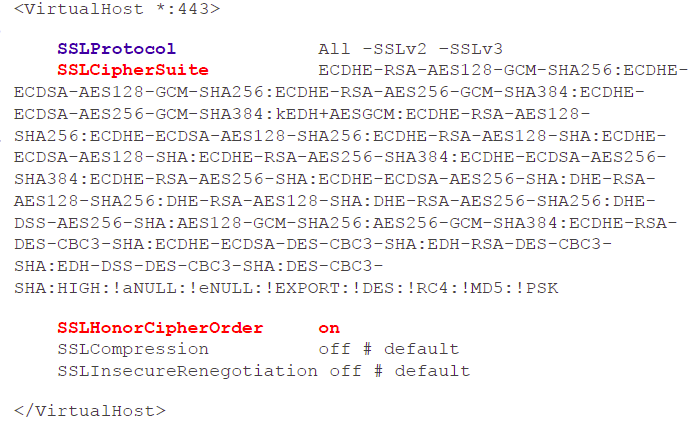
\includegraphics[width=0.8\textwidth]{./img/apache_ssl_configuration.png}
	\caption{Apache SSL Configuraiton}
\end{figure}

\subsubsection{Apache SSL Cipher Forwarding}
Der Vorteil dieser Variante ist, dass auch ältere Browsers sich mit der Applikation verbinden können, da der Apache alle Ciphers akzeptiert.\\

Apache leitet dann die SSL Informationen zu der Applikation,  via dem mod\_header weiter, welche dann den Entscheid für die entsprechende SSL Cipher Suit macht.
\begin{easylist}
	& Applikation muss die Cipher prüfen
	& Bei Änderungen oder neuen Cipher muss die Applikation neu konfiguriert werden.
\end{easylist}	



\end{document}